\subsection{Gestion des abonnements}
Cette partie va présenter toutes les fonctionnalités relatives à la consultation, la modification et la souscription à un abonnement. Du point de vue des utilisateurs, tous (y compris les visiteurs) ont accès à la consultation des offres (formules et forfaits étrangers). Par contre, un client à accès en plus à un résumé de ses achats (téléphone et formules).

\subsubsection{La liste des formules}
Cette vue est la principale associée à la gestion des abonnements. Elle présente un résumé de la liste des formules proposés par Centrale-Télécom. Le tableau présente donc les principales caractéristiques des formules, à savoir :
\begin{itemize}
  \itemperso{Nom et tarif}Les informations basiques pour que les utilisateurs se repèrent dans les formules.
  \itemperso{Promotion}Cette valeur est mise à \og Oui\fg{} si la formule est une promotion, \og Non\fg{} sinon.
  \itemperso{Téléphone associé}L'icône permet de savoir si la formule est associée à un ou plusieurs téléphones. Ceci permet de représenter les liens (par exemples promotionnels) entre une formule et un téléphone. Si un ou deux téléphones sont associés, alors l'icône est \vColor{\faMobilePhone}, sinon il s'agit de \thColor{\faMobilePhone}.
  \itemperso{Forfaits étrangers}Tout comme le champs sur les téléphones, il permet de savoir si l'offre est associée à une formule vers l'étranger. Ici aussi, si un ou plusieurs forfaits étrangers sont inclus dans la formule, alors l'icône est \vColor{\faGlobe}, sinon il s'agit de \thColor{\faGlobe}.
  \itemperso{Boutons d'édition}Ces boutons ne sont accessibles qu'en tant qu'administrateur.
\end{itemize}
Ces différents éléments peuvent être observés à la Figure~\ref{fig:liste-formule} qui propose la situation en tant qu'administrateur (avec les boutons d'édition et de création de formule).

\begin{figure}[ht]
  \centering
  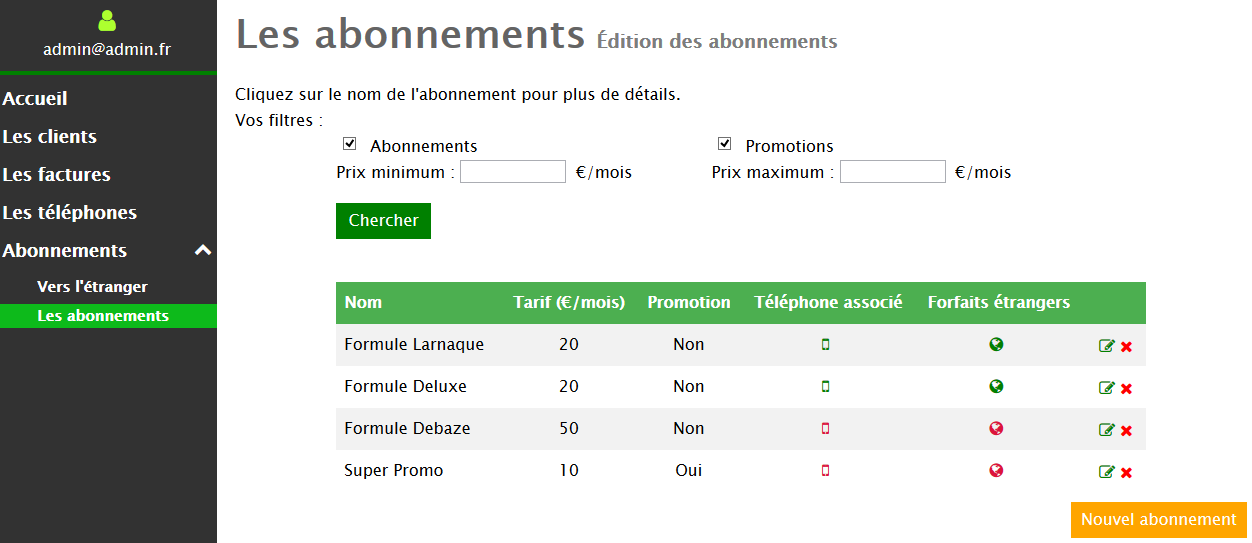
\includegraphics[width=.7\textwidth]{images/Plateforme/liste_formule}
  \caption{Vue présentant la liste des formules de Centrale-Télécom}
  \label{fig:liste-formule}
\end{figure}

Dans la suite, nous allons détailler les différentes actions possibles dans cette vue.

\subsubsection{Consultation des détails d'une formule}
\subParagraphe{Détails généraux}Si la table présentée à la Figure~\ref{fig:liste-formule} permet de visualiser les fondamentaux des formules, plus de détails sont disponibles pour ces dernières. Ainsi, en cliquant sur le nom de la formule (par exemple sur \og Super Promo\fg), on obtient une fenête modale qui présente les détails de la formule, comme proposé à la Figure~\ref{fig:details-formule}.

\begin{figure}[ht]
  \centering
  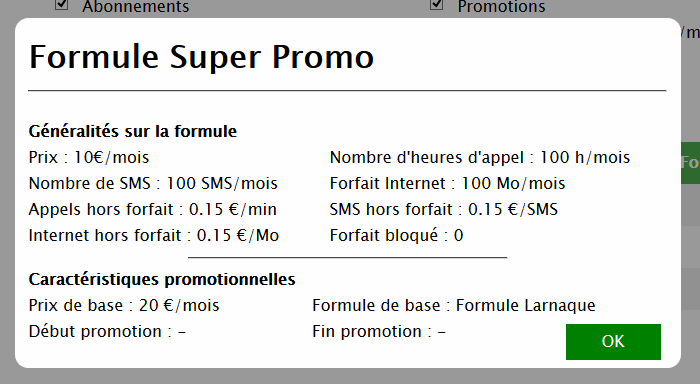
\includegraphics[width=.5\textwidth]{images/Plateforme/detail_formule}
  \caption{Détails d'une formule}
  \label{fig:details-formule}
\end{figure}

On remarquera en particulier que cette formule est une promotion sur la \og Formule Larnaque\fg{} et que les informations initiales de cette formule sont remontées.

Cette fonctionnalité est accessible à tous les utilisateurs.

\subParagraphe{Téléphones associés à la formule}En cliquant sur l'icône \faMobilePhone{}, on peut consulter la liste des téléphones qui sont associés à la formule. Ces téléphones peuvent par exemple bénéficier de tarifs préférentiels si on achète cette formule (ceci n'a pas été matérialisé dans la base de données cependant). Un exemple vous est proposé à la Figure~\ref{fig:telephones-associes}, où on peut visualiser que la \og Formule Larnaque\fg{} est associée à un téléphone.

\begin{figure}[ht]
  \centering
  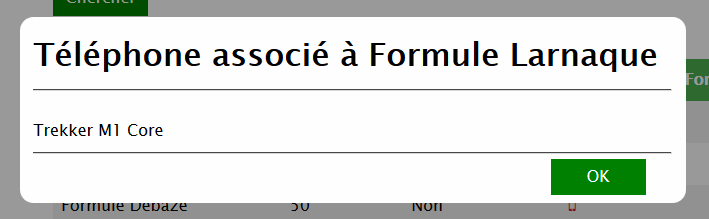
\includegraphics[width=.5\textwidth]{images/Plateforme/telephones_associes}
  \caption{Téléphone(s) associé(s) à la \og Formule Larnaque\fg}
  \label{fig:telephones-associes}
\end{figure}

On remarquera que cette vue est uniquement consultative, et que pour plus de détails, il est nécessaire de se rendre à la page de description des téléphones.

\subParagraphe{Forfaits étrangers associés à la formule}Pour obtenir la liste des forfaits étrangers associés à une formule, il suffit (de manière similaire aux téléphones associés), de cliquer sur l'icône \faGlobe{} qui va alors ouvrir une modale avec la liste des forfaits étrangers compris dans la formule. Un exemple vous est proposé à la Figure~\ref{fig:foreign-associes}.

\begin{figure}[ht]
  \centering
  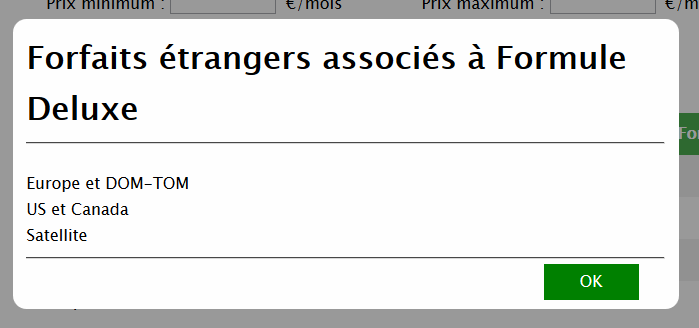
\includegraphics[width=.5\textwidth]{images/Plateforme/foreign_associes}
  \caption{Forfait(s) étranger(s) associé(s) à la \og Formule Deluxe\fg}
  \label{fig:foreign-associes}
\end{figure}

\subParagraphe{Recherche avancée}Afin de pouvoir plus facilement cibler une formule, nous avons mis en place quelques éléments de recherche pour les principaux critères. Il est ainsi possible de lancer une recherche en spécifiant un prix minimum et un prix maximum. Il est également possible de filtrer les résultats selon qu'il s'agisse d'offres promotionnelles, ou d'offres non-promotionnelles ou des deux.

Sur la base de tests qui vous a été fournis, on peut par exemple demander les offres non promotionnels ayant un tarif entre 15 et 25 euros. On obtient alors le résultat de la Figure~\ref{fig:filtrage-resultats}.

\begin{figure}[ht]
  \centering
  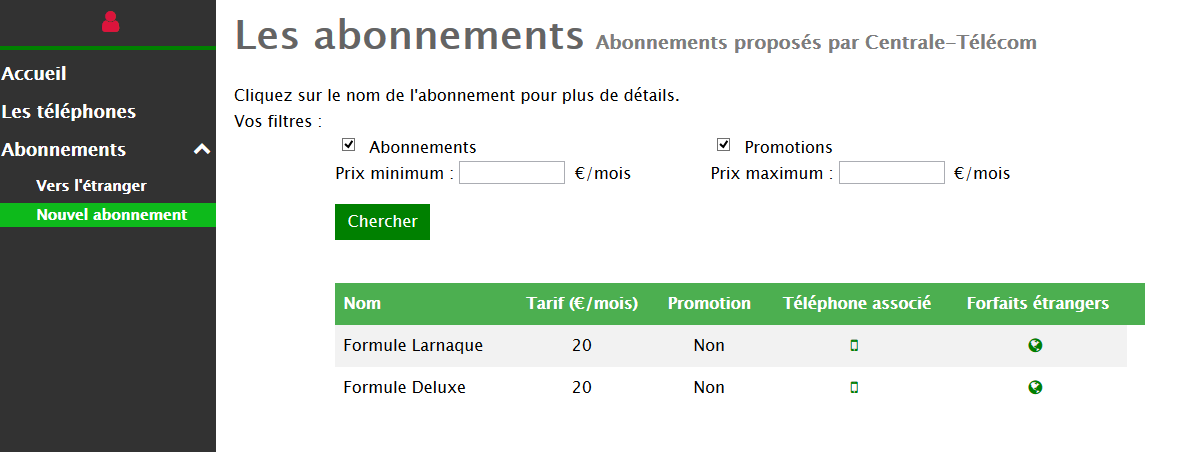
\includegraphics[width=.7\textwidth]{images/Plateforme/filtrage-resultats}
  \caption{Filtrage des formules avec l'outil de recherche}
  \label{fig:filtrage-resultats}
\end{figure}

\subsubsection{Consultation des forfaits étrangers}
La consultation des forfaits étrangers se fait selon les mêmes modalités que les formules tradionelles. On retrouve cependant moins de caractéristiques pour ces derniers. En effet, ils ne sont pas associés à des téléphones, ainsi, leurs principales caractéristiques sont juste des tarifs et des zones géographiques visées. La consultation de la liste est alors immédiate (Figure~\ref{fig:liste-etrangers}), et les détails sur une formule sont également obtenus en cliquant sur son nom (Figure~\ref{fig:details-etrangers}).

\begin{figure}[ht]
  \centering
  \begin{subfigure}{.57\textwidth}
    \centering
    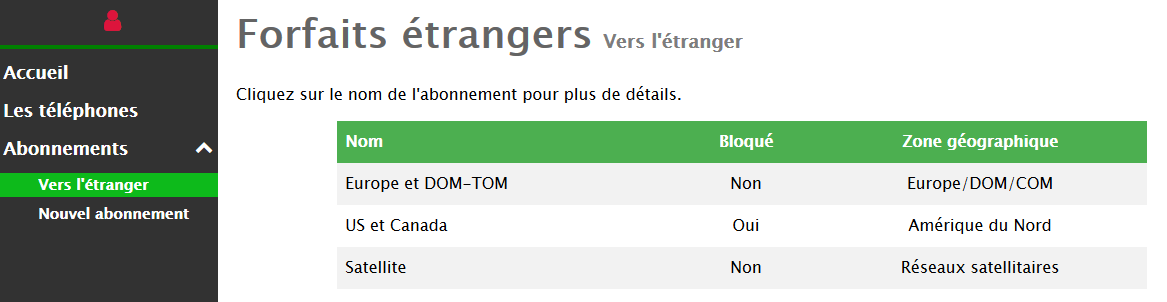
\includegraphics[width=\textwidth]{images/Plateforme/liste_etrangers}
    \caption{Liste des forfaits vers l'étranger}
    \label{fig:liste-etrangers}
  \end{subfigure}\hfill%
  \begin{subfigure}{.4\textwidth}
    \centering
    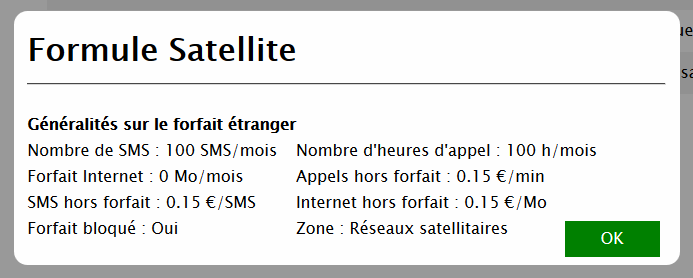
\includegraphics[width=\textwidth]{images/Plateforme/details_etranger}
    \caption{Liste des forfaits vers l'étranger}
    \label{fig:liste-etrangers}
  \end{subfigure}
  \caption{Consultation de la liste des forfaits étrangers et de leurs détails}
\end{figure}

Ici aussi, cette consultation est accessible à tous les niveaux d'utilisateur.

\subsubsection{Création, édition et suppression d'une formule ou d'un forfait étranger}
Ces fonctionnalités ne sont accessibles qu'aux administrateurs. Pour cela, ces derniers doivent se rendre dans les vues listant les offres (formules ou forfaits étrangers). Pour l'exemple, nous prendrons le cas des formules (qui est un peu plus sophystiqué).

\subParagraphe{Création d'une formule}Pour cela, l'administrateur doit cliquer sur le bouton \og Nouvel abonnement\fg. La modale de la Figure~\ref{fig:nouvel-abonnement} apparaît alors et lui permet de configurer cet abonnement.

\begin{figure}[ht]
  \centering
  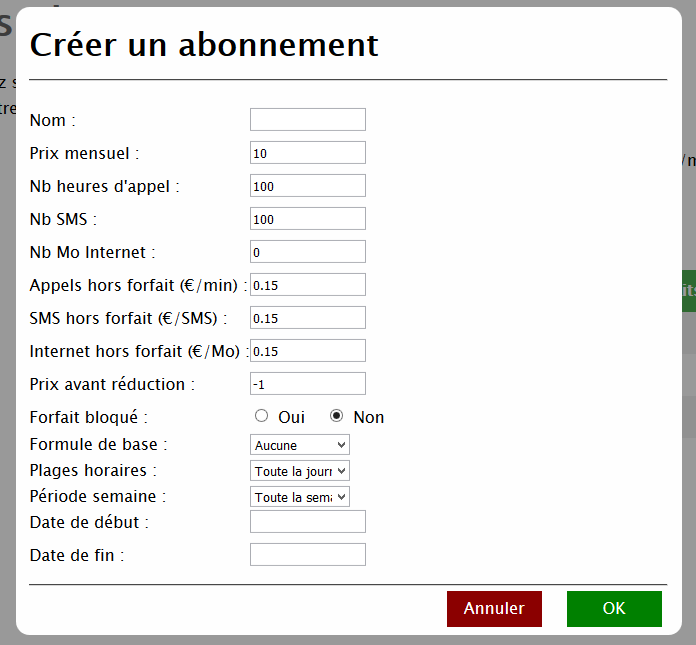
\includegraphics[width=.7\textwidth]{images/Plateforme/nouvel-abonnement}
  \caption{Modale de création d'un nouvel abonnement}
  \label{fig:nouvel-abonnement}
\end{figure}

Outre les champs classiques comme les prix ou les limites de consommation, on retrouve certains champs dépendant directement des informations stockées en base de données, comme la formule de base utilisée à partir de laquelle on applique une réduction. On remarquera l'absence des forfaits étrangers et des portables associés, qui pour des raison de facilité de code côté utilisateur ont été déportées dans des modales particulières.

\subParagraphe{Associer des forfaits étrangers à la formule}Pour cela, l'administrateur doit cliquer sur l'icône \faGlobe. À la différence de la modale précédemment sélectionnée, celle de l'administrateur permet de (dé)sélectionner les abonnements à inclure ou non dans la formule (Figure~\ref{fig:assoc-foreign}). Le changement est immédiat s'il clique sur \og OK\fg.

\subParagraphe{Associer des portables à la formule}Le fonctionnement est le même que pour les forfaits étrangers, mais en cliquant désormais sur \faMobilePhone{} (Figure~\ref{fig:assoc-telephone}).

\begin{figure}[ht]
  \centering
  \begin{subfigure}{.57\textwidth}
    \centering
    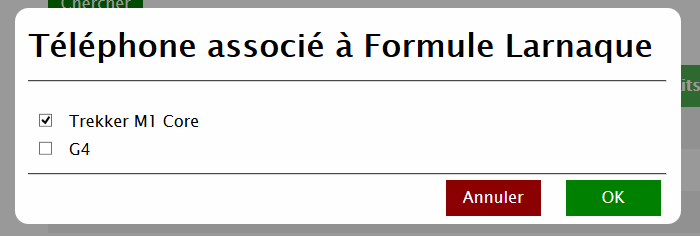
\includegraphics[width=\textwidth]{images/Plateforme/assoc_telephone}
    \caption{Téléphones}
    \label{fig:assoc-telephone}
  \end{subfigure}\hfill%
  \begin{subfigure}{.4\textwidth}
    \centering
    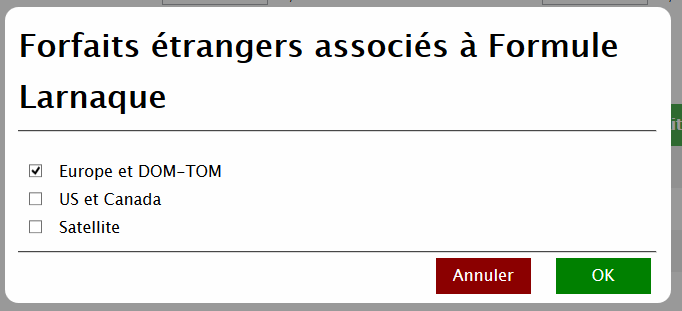
\includegraphics[width=\textwidth]{images/Plateforme/assoc_foreign}
    \caption{Forfaits étrangers}
    \label{fig:assoc-foreign}
  \end{subfigure}
  \caption{Modale pour associer des éléments à une formule}
\end{figure}

\subParagraphe{\'Edition d'un forfait}Pour éditer les champs remplis à la création du forfait (voir Figure~\ref{fig:nouvel-abonnement})

%%% Local Variables:
%%% mode: latex
%%% TeX-master: "../../Rapport_BDD"
%%% End:
